\documentclass[12pt, a4paper]{report}
\usepackage{graphicx}
\usepackage{ctex}
\usepackage[colorlinks=true]{hyperref}
\usepackage{indentfirst}
\usepackage{listings}
\graphicspath{{chapter/}{figures/}}
\usepackage{CJK}
\usepackage{tikz}
\usetikzlibrary{arrows,automata}
\usepackage{amsmath}

\usepackage{minted}

\begin{document} 
%%%%%%%%%%%%%%%%%%%%%%%%%%%%%%
%% 封面部分
%%%%%%%%%%%%%%%%%%%%%%%%%%%%%%
\begin{titlepage}
	\centering
	
\includegraphics[width=0.2\textwidth]{sf1.png}\par
	\vspace{1cm}
	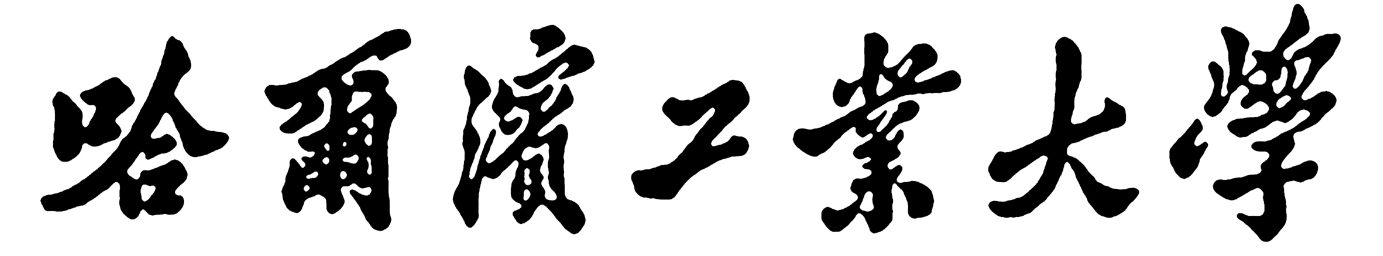
\includegraphics[width=0.8\textwidth]{sf.jpg}\par
	\vspace{0.1cm}
	{\scshape\LARGE Harbin Institute of Technology \par}
	\vspace{1cm}
	{\kaishu\LARGE 模式识别与深度学习\\实验报告\par}
	\vspace{1.5cm}
	{\huge\bfseries 对抗式生成网络\par}
	\vspace{2cm}
	{\fangsong\Large\itshape 黄海\par}
	\vfill
	{1160300329}\par
	\fangsong{计算机科学与技术}
	\vfill
	指导教师	\textsc{左旺孟}
	\vfill
% Bottom of the page
	{\large \today\par}
\end{titlepage}

\sc
\tableofcontents
\newpage

\chapter{最基本的GAN}
\section{原理}

对抗式生成网络,顾名思义,需要最基本的两个部件来进行生成,即生成器和判别器。
在给定true data的条件下,生成fake data提供给判别器,进行对抗。GAN的难点在于
调参,使两者中的任何一个都不会训练过头。

\section{代码}

以下是训练的部分代码
\small
\begin{minted}{python}

def gan_train(self):
    plt.ion()
    f, ax = plt.subplots(figsize=(8, 8))
    b_data = self.get_data()
    X, Y = np.mgrid[-1:2:complex(0, 100), -1:2:complex(0, 100)]
    print('Start Generator Trainning:')
    for step in range(steps):
        print('This is step:', str(step + 1))
        generator_ideas = Variable(torch.randn(8192, g_input_size))
        generator = self.G(generator_ideas)
        generator_points = generator.detach().numpy()
        prob_art_first = self.D(self.art)
        prob_art_second = self.D(generator)
        discriminator_loss = - torch.mean(torch.log(prob_art_first) 
                              + torch.log(1 - prob_art_second))
        generator_loss = torch.mean(torch.log(1 - prob_art_second))
        self.d_optimizer.zero_grad()
        discriminator_loss.backward(retain_graph=True)
        self.d_optimizer.step()
        self.g_optimizer.zero_grad()
        generator_loss.backward(retain_graph=True)
        self.g_optimizer.step()
        if step % 100 == 99:
            b_output = self.D(b_data).data.numpy()
            b_output = np.reshape(b_output, (100, 100))
            original_data = pd.DataFrame(Data().mat_data, 
                                          columns=['x', 'y'])
            output_data = pd.DataFrame(generator_points, columns=['x', 'y'])
            ax.set_xlim([-1, 2])
            ax.set_ylim([-1, 2])
            ax.set_title('GAN:This is step:' + 
                        str(step + 1), 
                        color='red', fontweight=800)
            pcm = ax.pcolor(X, Y, b_output, cmap=s)
            bar = f.colorbar(pcm, ax=ax)
            ax = sns.scatterplot(x='x', y='y', 
                      data=original_data, marker='X', color='b', s=30)
            ax = sns.scatterplot(x='x', y='y', 
                      data=output_data, marker='P', color='r', alpha=0.5, s=30)
            f.savefig('./results/Adam/GAN/step' 
                      + str(step+1) + '.png')
            plt.pause(0.05)
            bar.remove()
    plt.ioff()
    f.show()

\end{minted}

\normalsize
\section{实验结果}

\begin{figure}[ht]
  \centering
  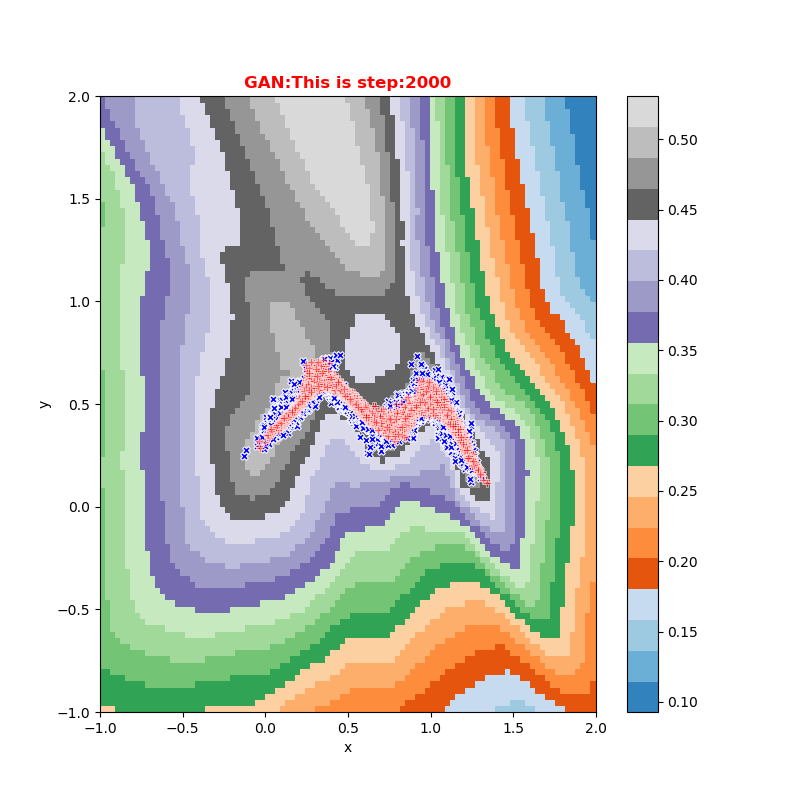
\includegraphics[scale=0.6]{figure1.png}
  \caption{GAN训练结果}
  \label{}
\end{figure}

\chapter{WGAN}

\section{解释}

GAN的难点也是自己的不足,两个部件很难训练到一个恰当的程度。这个问题产生的根本在于生成的noise和真正的
true data之间的联系权重过高,使得判别器有一丁点的改动生成器就会过度反应。解决的方法在于为参数进行减权,
即在判别器更新之后,对参数赋予一个权重系数。

WGAN个GAN的区别主要存在于以下四点
\begin{enumerate}
  \item loss函数不需要进行对数操作
  \item 网络中判别器最后不需要Sigmod
  \item 对参数赋予权重
  \item 不使用基于动量的优化算法
\end{enumerate}

\section{代码}

以下展示了于GAN不同的地方
\small
\begin{minted}{python}
# 没有sigmod
class WGANDiscriminator(nn.Module):
    def __init__(self):
        super(WGANDiscriminator, self).__init__()
        self.n1 = nn.Linear(d_input_size, d_hidden_size)
        self.n2 = nn.Linear(d_hidden_size, d_hidden_size)
        self.n3 = nn.Linear(d_hidden_size, d_return_size)
        self.relu = nn.ReLU()
        # self.sig = nn.Sigmoid()

    def forward(self, x):
        x = self.relu(self.n1(x))
        x = self.relu(self.n2(x))
        x = self.n3(x)
        return x

# loss函数
discriminator_loss = - torch.mean(prob_art_first + 1 - prob_art_second)
generator_loss = torch.mean(1 - prob_art_second)

# 优化器
self.d_optimizer = optim.RMSprop(self.D.parameters(), lr=d_lr)
self.g_optimizer = optim.RMSprop(self.G.parameters(), lr=g_lr)

# 参数截断
for i in self.D.parameters():
    i.data.clamp_(-c, c)

\end{minted}

\normalsize

\section{结果}

\begin{figure}[ht]
  \centering
  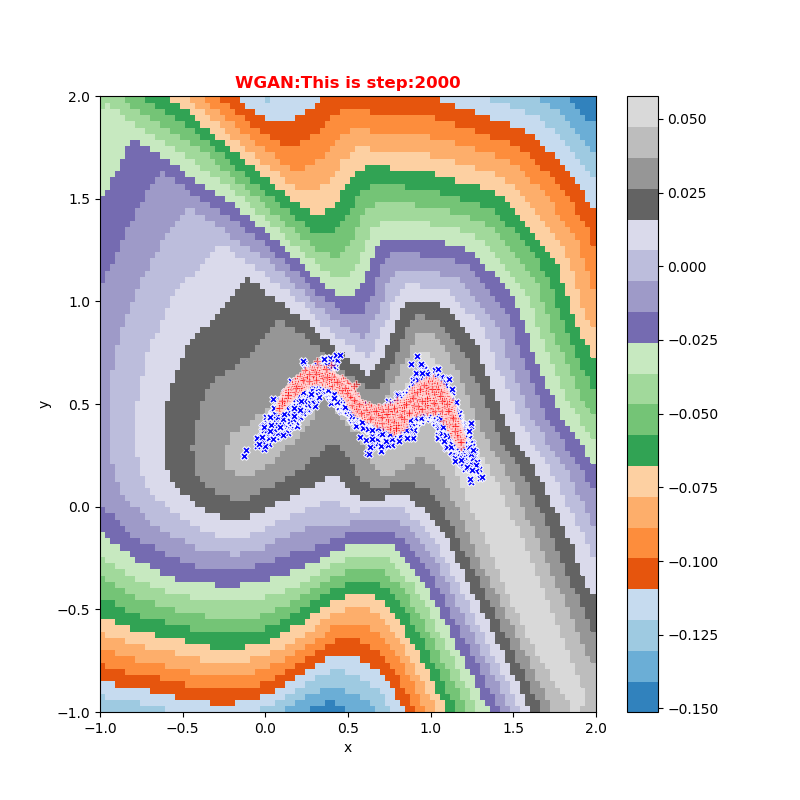
\includegraphics[scale=0.6]{figure2.png}
  \caption{WGAN训练结果}
  \label{}
\end{figure}

\chapter{WGAN-GP}

\section{解释}

WGAN解决了部分训练过度的问题,但是也暴露出其他的缺点,例如收敛过慢,在精细调参后的效果不如GAN等等。
WGAN-GP有解决了这类问题,对于WGAN,只需要对梯度进行更改。这里需要有梯度惩罚措施,加快收敛速度但是不至于
过快的下降。

\section{代码}

以下展示了于WGAN不同的地方
\small
\begin{minted}{python}
# 梯度惩罚
def calc_gradient_penalty(self, netD, real_data, fake_data):
    # print real_data.size()
    alpha = torch.rand(8192, 1)
    alpha = alpha.expand(real_data.size())
    interpolates = alpha * real_data + ((1 - alpha) * fake_data)
    interpolates = autograd.Variable(interpolates, requires_grad=True)
    disc_interpolates = netD(interpolates)
    gradients = autograd.grad(outputs=disc_interpolates, inputs=interpolates,
              grad_outputs=torch.ones(
              disc_interpolates.size()),
              create_graph=True, retain_graph=True, only_inputs=True)[0]
    gradient_penalty = ((gradients.norm(2, dim=1) - 1) ** 2).mean() * LAMBDA
    return gradient_penalty
\end{minted}

\normalsize

\section{结果}

\begin{figure}[ht]
  \centering
  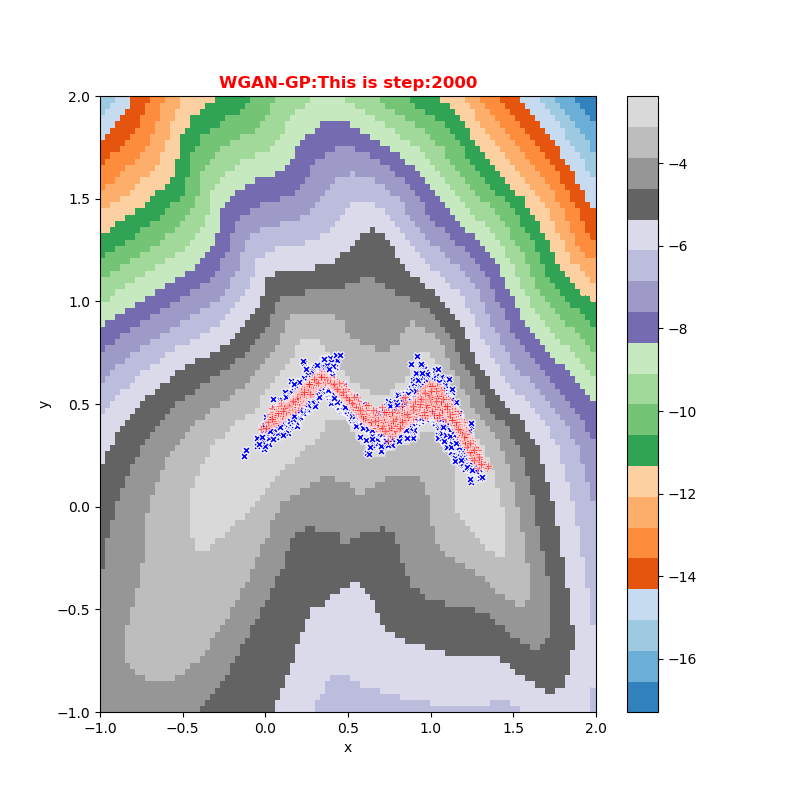
\includegraphics[scale=0.6]{figure3.png}
  \caption{WGAN-GP训练结果}
  \label{}
\end{figure}

\end{document}
